
%%% Local Variables: 
%%% mode: latex
%%% TeX-master: t
%%% End: 
\documentclass[twocolumn]{article}



% My mom is always telling me that, a man has to learn to do some
% basic house keeping. Or he shall never turn a good man.
\usepackage{amsmath}
\usepackage{amssymb}
\usepackage[margin=10mm]{geometry}
\usepackage{graphicx}
\graphicspath{{./}{./Figures/}}
\usepackage{algorithm}
\usepackage{algorithmic}


\begin{document}
\begin{itemize}
\item \textbf{CIA}, a modern definition. Confidentiality: prevent
  unauthorized reading of information. Integrity: detect unauthorized
  writing of information. Availability: data is available in a timely
  manner when needed. 
\item \textbf{Network Security}. Various protocols play a critical
  role, and cryptography matters a lot in protocol (especially network
  protocols) design and analysis.
\item \textbf{Kerckhoof's Principle}. The system is completely known
  to the attacker; only the key is secret; the crypto algorithms are
  not secret. 
\item \textbf{Confusion and Diffusion}. Confusion: obscuring the
  relationship between plaintext and ciphertext. Diffusion: spreading
  the plaintext statistics through the ciphertext. A little note: hash
  function can be viewed as \emph{one way cryptography}.
\item \textbf{Stream Cipher}. Both A5/1 and RC4 are examples of this
  symmetric cryptosystem. It generalized the idea of a one-time pad,
  except that we trade provably security with a relatively small (and
  manageable) key. The key is stretched into a long stream of bits,
  which is then used just like a one-time pad. 
\item \textbf{Block Cipher}. It's really just an ``electronic''
  version of a codebook, and employs both confusion and diffusion. 
  % \begin{algorithm}
  %   \begin{algorithmic}
  %     \STATE~Life is a bitch.
  %     \IF{You are a bitch}
  %     \STATE~Do something never that silly.
  %     \ENDIF
  %   \end{algorithmic}
  % \end{algorithm}
  \begin{algorithm}
    \caption{RC4 Keystream Byte}
    \label{algo:rc4-keystream-byte}
    \begin{algorithmic}
      \STATE~$i=(i+1)\mod 256$
      \STATE~$j=(j+S[i]\mod 256)$
      \STATE~swap $(S[i], S[j])$
      \STATE~$t=(S[i]+S[j]\mod 256)$
      \STATE~$Keystream~ byte=S[t]$
    \end{algorithmic}
  \end{algorithm}
\item \textbf{Feistel Cipher}. It's a general cipher design
  principle. $L_{i}=R_{i-1}$ and $R_{i}=L_{i-1}\oplus
  F(R_{i-1},K_{i})$.
\item \textbf{DES}. The security of this cryptosystem has much to do
  with \emph{S-box}. Steps: an initial permutation before round 1;
  halves are swapped after last round; a final permutation applied to
  $R_{16},L_{16}$. 
  \begin{algorithm}
    \caption{TEA Encryption}
    \label{algo:tea-encryption}
    \begin{algorithmic}
      \STATE~$(K[0],K[1],K[2],K[3])=128~bit~key$
      \STATE~$(L,R)=plaintext$ ($64-bit$ block)
      \STATE~$delta=0$x$9e3779b9$
      \STATE~$sum=0$
      \FOR{$i=1$ to $32$}
      \STATE~$sum=sum+delta$
      \STATE~$L=L+(((R\ll 4)\oplus K[0])\oplus (R+sum)\oplus ((R\gg
      5)\oplus K[1]))$
      \STATE~$R=L+(((L\ll 4)\oplus K[2])\oplus (L+sum)\oplus ((L\gg
      5)\oplus K[3]))$
      \STATE~next $i$
      \ENDFOR
      \STATE~$ciphertext=(L,R)$
    \end{algorithmic}
  \end{algorithm}
\item \textbf{Block Cipher Modes}. ECB:\@ encrypt each block
  independently. CBC:\@ chain the blocks together. For this mode, a
  random initialization vector is required. CTR:\@ block cipher acts
  like stream one.  
\item \textbf{Data Integrity}. The encryption process does provide
  confidentiality, but no guarantee of integrity. 
  \begin{algorithm}
    \begin{algorithmic}
      \caption{Key generation for RSA public key encryption}
      \label{algo:keygen-for-rsa-encrypt}
      \ENSURE~Each entity creates an RSA public key and a
      corresponding private key. Each entity A should do the
      following:
      \begin{enumerate}
      \item Generate two large random and distinct primes $p$ and $q$,
        each roughly the same size.
      \item Compute $n=pq$ and $\phi=(p-1)(q-1)$.
      \item Select a random integer $e$, $1\leq e\leq\phi$, such that
        $\gcd(e,\phi)=1$. 
      \item Use the extended Euclidean algorithm to compute the unique
        integer $d$, such that $ed\equiv 1\mod\phi$.
      \item A's public key is $(n,e)$, private key is $d$.
      \end{enumerate}
    \end{algorithmic}
  \end{algorithm}
\item \textbf{RSA Validity Proof}.
  \begin{itemize}
  \item Since $ed\equiv 1\mod\phi$, there exists an integer $k$ such
    that $ed=1+k\phi$. 
  \item Now if $\gcd(m,p)=1$, then by Fermat's theorem, $m^{p-1}\equiv
    1\mod p$. 
  \item Raising both sides of this congruence to the power $k(q-1)$
    and then multiplying both sides by $m$ yields
    $m^{1+k(p-1)(q-1)}\equiv m\mod p$.
  \item On the other hand if $\gcd(m,p)=p$, then this last congruence
    is valid since each side is congruence to $0\mod p$. 
  \item Hence, in all cases, $m^{ed}\equiv m\mod p$. By the same
    argument, $m^{ed}\equiv m\mod q$. 
  \item Finally, since $p$ and $q$ are distinct primes, it follows
    that $m^{ed}\equiv m\mod n$. And hence, $c^{d}\equiv
    {(m^{e})}^{d}\equiv m\mod n$.
  \end{itemize}
\item \textbf{Cube Root attack} on RSA.\@ A simple but practical way to
  prevent is to pad message with random bits.
\item \textbf{Cryptographic Hash Function}. This function must provide
  the following:
  \begin{itemize}
  \item Compression. For any size input $x$, the output length,
    i.e. $h(x)$ is small. Usually a fixed length is pre-defined.
  \item Efficiency. It must be easy to compute $h(x)$ for any input
    $x$. 
  \item One way. Given any value $y$, it's computationally infeasible
    to find a value $x$ such that $h(y)=x$.
  \item Weak Collision Resistance. Given $x$ and $h(x)$, it's
    infeasible to find any $y$, with $y\neq x$, such that
    $h(y)=h(x)$.
  \item Strong Collision resistance. It's (and should be so)
    infeasible to find any $x\neq y$ such that $h(x)=h(y)$.
  \end{itemize}
\item \textbf{Birthday Problem}. Strong one. How large much the $N$ be
  before the probability that someone shares the same birthday with
  me? Weak one. How many people must be in a room before the
  probability of at least two share the same birthday is larger than
  $0.5$?  
\item \textbf{Access Control}. Two easy-to-understand
  comparisons. Authentication: are you who you say you are?
  Authorization: are you allowed to do that fucking (forgive my
  rudeness; I am tired.) stuff?
\item \textbf{Common Attacks on Passwords}. Usually, this applies to
  many other similar stuff in security as well. Outsider, and then you
  ``act as if'' you are a normal user. Some time when ``the day''
  comes, you may have the privilege to ``self-promoting'' to (one of)
  the administrators.
\item \textbf{Iris Scan Attacks}. One thing pointed out in the slides,
  ``scanners could use light to'' make sure that it's scanning a live
  eye. 
\item \textbf{Web Cookies}. According to our official textbook, web
  cookies have ``some interesting security implications''. Web cookie
  is simply a numerical value that is stored and managed by one's
  browser. The website that one is visiting also stores the cookie,
  which is used to index a database that retains information about
  Alice (in textbook flavor). In a slightly stronger ``expression'', a
  password is used to initially authenticate Alice, after which the
  cookie is considered sufficient.
\item \textbf{Evaluation Assurance Level}. Note that a product with a
  higher EAL does not necessarily mean it \emph{does} possess a higher
  security power (forgive me for the lack of words). For example,
  suppose that product A is certificated EAL4, while product B carries
  EAL5 rating. All it means is that product A was evaluated for EAL4
  (and passed), while product B was actually evaluated for EAL5 (and,
  at the same time, passed). It is possible that product A could have
  achieved EAL5 or higher, but the developers simply felt it was not
  worth the cost and effort to try a higher EAL.\@
\item \textbf{Classification and Clearances}. Classification applies
  to \emph{objects}. Clearance applies to \emph{subjects}. 
\item \textbf{Compartments}. They serve to enforce the \emph{need to
    know} principle, that is, subjects are only allowed to know the
  information that they \emph{must} know for their work.
\item \textbf{Covert Channel}. Three things are required for a covert
  channel to exist. First, the sender and receiver must have access to
  a shared resource. Second, the sender must be able to vary some
  property of the shared resource that the receiver can
  observe. Finally, the sender and receiver must be able to
  synchronize their communication. 
\item \textbf{CATPCHA} Completely Automated Public Turing test to tell
  Computers and Humans Apart. It is a program that can generate and
  grade tests that it itself cannot pass. (Indeed much like some
  professors, or a lot of professors, in China.)
% I love programming, and I love Computer Science. That's why I am at
% Abu Dhabi. (Partially).
\item \textbf{Firewall}. In computing, a firewall is a software or
  hardware-based network security system that controls the incoming
  and outgoing network traffic by analyzing the data packets and
  determining whether they should be allowed through or not, based on
  applied rule sets. (Firewall can be defined in many ways according
  to your level of understanding.) A firewall establishes a barrier
  between a trusted, secure internal network and another network
  (well, take our beloved Internet for example) that is \emph{not
    assumed to be} secure and trusted. 
\item \textbf{Packet Filter}. It works by inspecting the ``packets''
  which transfer between computers on the Internet. If a packet
  matches the packet filter's set of rules, the packet filter will
  drop the packet, or reject it. This type of packet filtering pays no
  attention to \emph{whether a packet is part of an existing stream or
  traffic}.
\item \textbf{Stateful Filter}. Its work is achieved by retaining
  packets until enough information is available to make a judgment
  about its state. Obviously, from the description above, we can infer
  that this sort of firewall works on the \emph{transport layer}.
\item \textbf{Proxy Server}. A proxy server is a gateway from one
  network to another for a specific network application, in the sense
  that it functions as a proxy on behalf of (most probably, inner)
  network users.
\item \textbf{Authenticate over Network}. For attackers, they can:
  passively observe messages; they can also \emph{replay} messages;
  they can also actively attack you, like insert, delete or change
  your messages. 
\item \textbf{Keys or Passwords}. Yet another time according to our
  beloved textbook. After all, passwords are a little more than a
  crutch used by \emph{humble humans} because most of the case we are
  incapable of remembering keys. That is, passwords are about the
  closest thing to a key that, \emph{a humble human being} can
  remember. So if Alice and Bob are ``actually machines'' (that's the
  case) in real world communications, they should use keys instead of
  password, as \emph{the} authentication tool.
\item \textbf{Authentication Using Symmetric Keys}. Final version as
  suggested by textbook. Encrypt the user's identity together with the
  nonce. In this manner, Trudy cannot use a response from Bob for the
  third message---or it ``seems'' that it's encrypted by Bob himself.
\item \textbf{Something more about Public Key}. As the concept in
  (modern) cryptography goes, ``the public key is public''. Or, should
  it be public? Should it be so public? Could it possibly be, say,
  private? 
\item \textbf{Authentication Using Session Keys}. Instead of signing
  \emph{or} encrypting the messages, we sign \emph{and} encrypt the
  message.
  \begin{figure}[htbp]
    \centering
    \label{fig:mutual-authentication-session-key}
    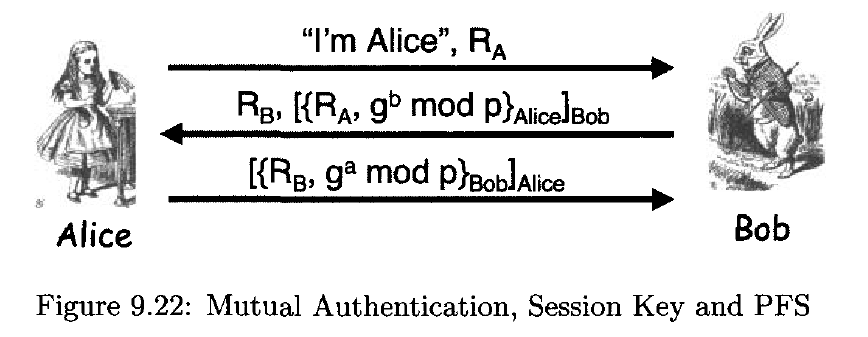
\includegraphics[scale=0.28]{Mutual-Authentication}   
  \end{figure}
\item \textbf{Public Key Authentication Drawback}. There may be one
  approach that is dangerous. If you encrypt your message with the
  other one's public key, and your time stamp is also included in this
  encryption. Later on you sign this specific message with your
  private key (aka, as the ``digital signature''). It may suffer
  attack! 
  \begin{figure}[htbp]
    \centering
    \label{fig:simplified-ssh}
    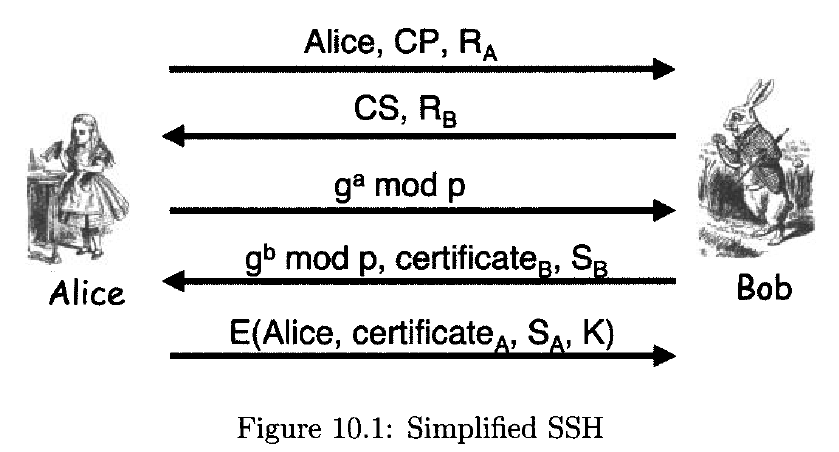
\includegraphics[scale=0.3]{Simplified-SSH}
  \end{figure}
\item \textbf{God Bless SSH}. Such a login typically requires a
  password and tools like \emph{rlogin} simply sends the password in
  the clear (aka, plaintext, or rather, message that can be
  eavesdropped easily), which might be observed by a snooping
  Trudy. By first establishing an SSH session, any inherently insecure
  command such as \emph{rlogin} will be secure. That is, an SSH
  session provides confidentiality and integrity protection.
  \begin{figure}[htbp]
    \centering
    \label{fig:simplified-ssl}
    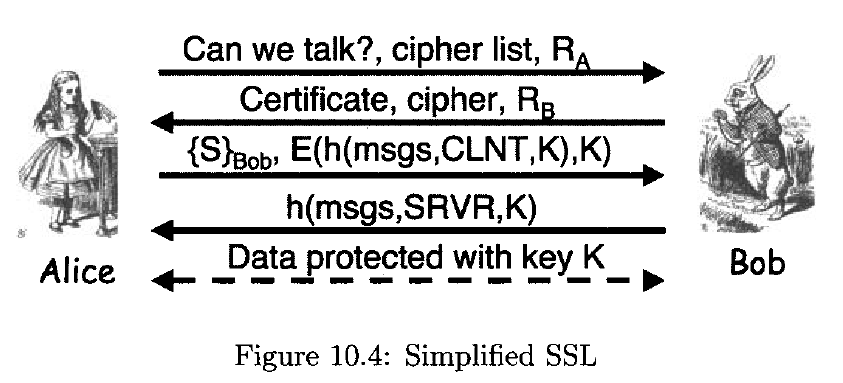
\includegraphics[scale=0.28]{Simplified-SSL}
  \end{figure}
  \begin{algorithm}
    \caption{Simple SSL in A Nutshell}
    \label{sec:simple-ssl-in-nutshell}
    \begin{algorithmic}[1]
      \STATE~Alice passes a list of ciphers that she supports, along
      with a nonce $R_{A}$.
      \STATE~Bob selects one of the ciphers from the cipher list that
      Alice sent in the message one, and he sends a nonce $R_{B}$.
      \STATE~Alice sends a pre-master secret $S$, along with a hash
      that is encrypted with the key $K$.
      \STATE~Bob responds with a similar hash.
      \STATE~At this point, Alice has authenticated Bob. And Alice and
      Bob has established a shared session key $K$.
    \end{algorithmic}
  \end{algorithm}

\item \textbf{SSL versus IPSec}. 
  \begin{itemize}
  \item SSL is very simple whereas IPSec is, well, indeed it is
    extremely complex.
  \item SSL lives at socket layer, thus residing is user space. IPSec
    lives at network layer and is therefore not directly accessible
    from user space---it's in the domain of \emph{the operating
      system}. 
  \item Both SSL and IPSec provide encryption, integrity protection,
    and authentication.
  \end{itemize}

\item \textbf{Internet Key Exchange}. Mutual authentication is
  supported. Session key should (and would) be established. Phase 1,
  IKE security association. Phase 2, AH/ESP security
  association. Something more: the main mode \emph{must} be
  implemented whereas the aggressive mode \emph{should} be
  implemented. 
\item \textbf{Transport and Tunnel Modes}. Independent of whether ESP
  or AH is used, IPSec employs either \emph{transport mode} or
  \emph{tunnel mode}. 
  \begin{itemize}
  \item In transport mode, the new ESP/AH header is sandwiched
    between the IP header and the data.
  \item Transport mode is more efficient since it adds a minimal
    amount of additional header information.
  \item The downside of transport mode is that a passive attacker can
    see the headers. This mode is mainly designed for host-to-host
    communication. 
    \begin{figure}[htbp]
      \centering
      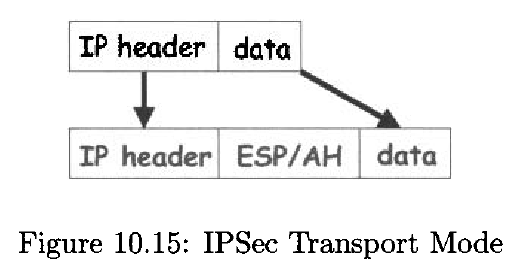
\includegraphics[scale=0.5]{IPSec-Transport-Mode}
    \end{figure}
  \item In tunnel mode,  the entire IP packet is encapsulated in a new
    IP packet. 
    \begin{figure}[htbp]
      \centering
      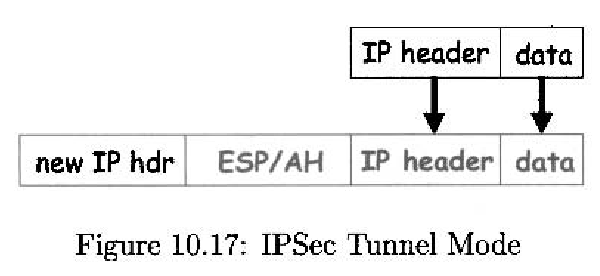
\includegraphics[scale=0.4]{IPSec-Tunnel-Mode}
    \end{figure}
  \end{itemize}

\item \textbf{AH versus ESP}. Authentication Header: provides only
  integrity. Encapsulating Security Payload: integrity and
  confidentiality are provided at the same time. For ESP, everything
  is protected \emph{except} IP header. 
\item \textbf{Buffer Overflow}. A buffer overflow must exist in the
  code. But not all buffer overflows are exploitable. However, if
  exploitable, the attacker can \emph{inject code}.
\item \textbf{Race Conditions}. To prevent race conditions, one option
  is to make security-critical processes \emph{atomic}.



\end{itemize}
\end{document}
     


